This chapter lists the requirements for an effect unit for a guitar. The requirements are based on the effect analysing and the Problem Statement.

\begin{figure}[htbp]
	\centering
\begin{picture}(0,0)%
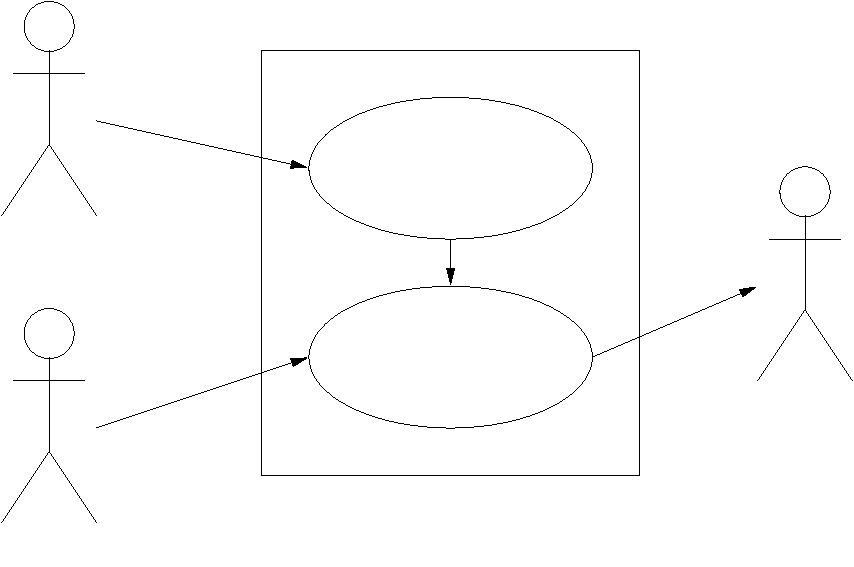
\includegraphics{Use_case.pdf}%
\end{picture}%
\setlength{\unitlength}{4144sp}%
%
\begingroup\makeatletter\ifx\SetFigFont\undefined%
\gdef\SetFigFont#1#2#3#4#5{%
  \reset@font\fontsize{#1}{#2pt}%
  \fontfamily{#3}\fontseries{#4}\fontshape{#5}%
  \selectfont}%
\fi\endgroup%
\begin{picture}(6507,4318)(1426,-4900)
\put(1531,-2491){User}%
\put(4546,-3346){Effect}%
\put(4276,-1906){Effect select}%
\put(7111,-3751){Amplifier}%
\put(1441,-4831){Guitar}%
\end{picture}%
	\caption{A graphically overview of wanted functionality in form of an use case digram.}
	\label{fig:use_case}
\end{figure}

The requirements are divided into unit, based on the effect analysing \autoref{ch:analysing}, where it is concluded in the \autoref{ch:analysing} that only 6 overall unit needs to be designed, and after this unit is designed, all effect can be made from this unit. The unit that needs to be designed is:


\begin{itemize}
	\item Bandpass filter
	\item Inverse bandpass filter
	\item Delay
	\item Gain
	\item Clipping
	\item \gls{lfo}
\end{itemize} 

 Besides each unit shall be designed individual, each unit interface shall fit to every effect where the unit is used. Each unit is divided intro its own section where the requirements are presented along with arguments for the requirement and a description of the requirement.
 
 